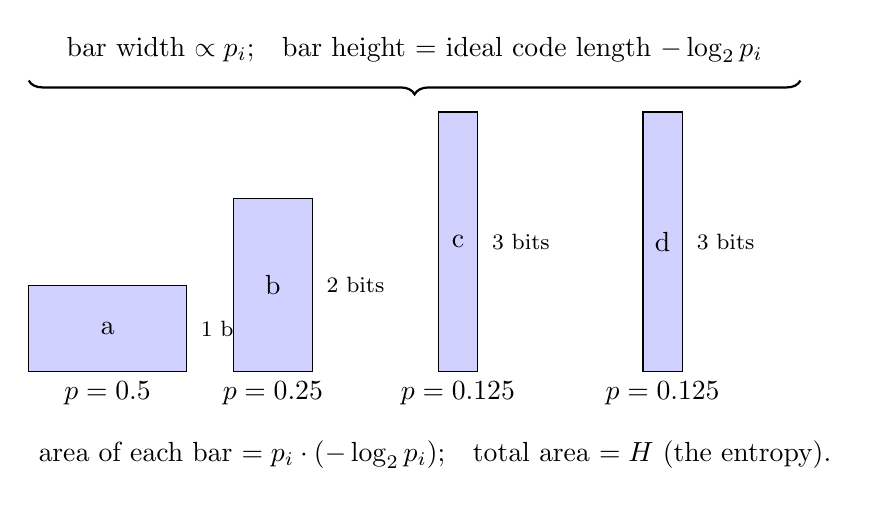
\begin{tikzpicture}[scale=1.0]
% colah-style: each symbol's bar shows -log2 p as its ideal code length.
% 4 symbols: p = 1/2, 1/4, 1/8, 1/8  -> lengths 1, 2, 3, 3
\foreach \i/\p/\len/\name in {0/0.5/1/a, 1/0.25/2/b, 2/0.125/3/c, 3/0.125/3/d}{
  \pgfmathsetmacro{\w}{4*\p}
  \draw[fill=blue!18] (\i*2.6,0) rectangle ({\i*2.6+\w},{1.1*\len});
  \node at ({\i*2.6+\w/2},{0.55*\len}) {\name};
  \node[below] at ({\i*2.6+\w/2},0) {$p=\p$};
  \node[right, font=\footnotesize] at ({\i*2.6+\w+0.06},{0.55*\len})
    {\len\ifnum\len>1 ~bits\else ~bit\fi};
}
\draw[decorate, decoration={brace, amplitude=5pt}, thick] (9.8,3.7) -- (0,3.7);
\node[align=center, above] at (4.9,3.8) {bar width $\propto p_i$;\quad
  bar height $=$ ideal code length $-\log_2 p_i$};
\node[align=left, anchor=north west] at (0,-0.75) {area of each bar
  $=p_i\cdot(-\log_2 p_i)$;\quad total area $=H$ (the entropy).};
\end{tikzpicture}
